\documentclass[tikz,border=10pt]{standalone}
% No extra libraries needed
\begin{document}
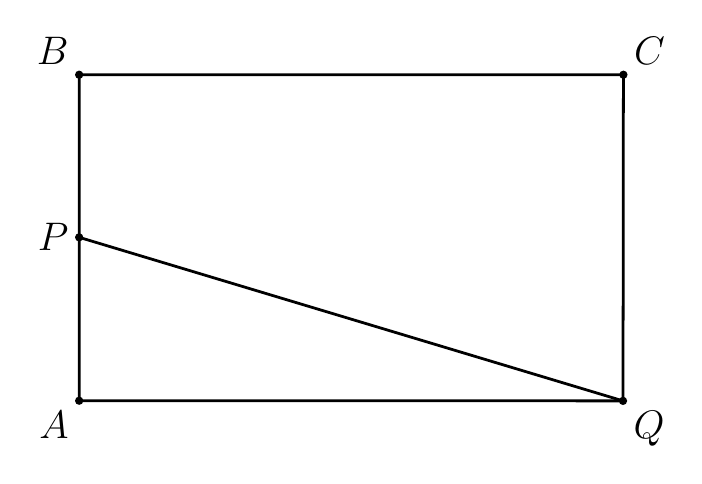
\begin{tikzpicture}[line join=round, line width=1.0pt]
  % Vertices: pixel coords scaled with s=0.017544, centre (265,183), y flipped
  \coordinate (B) at (-3.456, 2.070);
  \coordinate (C) at (3.456, 2.070);
  \coordinate (Q) at (3.451, -2.072);
  \coordinate (A) at (-3.456, -2.070);
  \coordinate (P) at (-3.456, 0.005);

  % Rectangle sides
  \draw (B) -- (C) -- (Q) -- (A) -- cycle;

  % Solid segment P to Q
  \draw (P) -- (Q);

  % Small dots at vertices
  \foreach \X in {A,B,C,P,Q}
    \fill (\X) circle (1.5pt);

  % Labels placed outside the figure
  \node[above left, font=\fontsize{14.5}{17.4}\selectfont] at (B) {$B$};
  \node[above right, font=\fontsize{14.5}{17.4}\selectfont] at (C) {$C$};
  \node[below left, font=\fontsize{14.5}{17.4}\selectfont] at (A) {$A$};
  \node[below right, font=\fontsize{14.5}{17.4}\selectfont] at (Q) {$Q$};
  \node[left, font=\fontsize{14.5}{17.4}\selectfont] at (P) {$P$};
\end{tikzpicture}
\end{document}